\documentclass[12pt]{article}
\usepackage[utf8]{inputenc}

% ============================================================================
% PACKAGE IMPORTS - Generally no need to modify unless adding new features
% ============================================================================
\usepackage{graphicx}
\usepackage{float}
\usepackage{caption}
\usepackage{subcaption}
\usepackage{geometry}
\geometry{a4paper, margin=0.8in}
\usepackage{amsmath, amsfonts, amssymb}
\usepackage{booktabs, array}
\usepackage{fancyhdr}
\usepackage{titlesec}
\usepackage{listings}
\usepackage{xcolor}
\usepackage[hidelinks]{hyperref}
\usepackage{enumitem}
\usepackage{cite}
\usepackage{cleveref}

\lstset{
  literate={β}{{$\beta$}}1
}


% Code listing style
\lstdefinestyle{pythonstyle}{
    language=Python,
    basicstyle=\ttfamily\scriptsize,
    keywordstyle=\color{blue}\bfseries,
    commentstyle=\color{green!50!black},
    stringstyle=\color{red},
    numberstyle=\tiny\color{gray},
    numbers=left,
    numbersep=5pt,
    frame=single,
    breaklines=true,
    breakatwhitespace=false,
    tabsize=2,
    showspaces=false,
    showstringspaces=false,
    captionpos=b,
    backgroundcolor=\color{gray!5},
    morekeywords={
        DataFrame, LinearRegression
    }
}


\lstset{style=pythonstyle}

% ============================================================================
% CUSTOMIZATION SECTION - EDIT THESE VARIABLES FOR YOUR ASSIGNMENT
% ============================================================================
% Replace the values below with your specific assignment details:

\newcommand{\universityname}{University of Moratuwa}                    % Your university name
\newcommand{\departmentname}{Department of Electronic and Telecommunication Engineering}  % Your department
\newcommand{\modulecode}{EN3150}                                        % Course/module code
\newcommand{\modulename}{Pattern Recognition}                    % Course/module name
\newcommand{\assignmentname}{Learning from data and related challenges and linear models}  % Your assignment title


% Page setup
% Page margins - adjust as needed (left, right, top, bottom)
\geometry{left=2.5cm, right=2.5cm, top=2.5cm, bottom=2.5cm}

% Header and footer setup
\pagestyle{fancy}
\fancyhf{}                        % Clear all header and footer fields
\fancyhead[L]{\modulecode}      % Left header: Module code and name
\fancyhead[R]{\assignmentname}               % Right header: Assignment name
\fancyfoot[C]{\thepage}                      % Center footer: Page number


% ============================================================================
% DOCUMENT CONTENT STARTS HERE
% ============================================================================
\begin{document}

% ============================================================================
% TITLE PAGE - Modify student information below
% ============================================================================
\begin{titlepage}
    \centering
    \vspace*{1cm}

    {\huge\textbf{\universityname}}\\[1cm]

    {\Large\textbf{\departmentname}}\\[0.5cm]

    
\includegraphics[width=0.5\textwidth]{resources/University_of_Moratuwa_logo.png}\\[1cm]

    {\large\textbf{\modulecode – \modulename}}\\[1cm]

    {\LARGE\textbf{\assignmentname}}\\[1cm]
    
    \vspace{0.3cm}
    
    % ========================================================================
    % STUDENT INFORMATION - CHOOSE ONE OPTION BELOW
    % ========================================================================
    
    % OPTION 1: FOR GROUP ASSIGNMENTS (Comment out Option 2 if using this)
    % \textbf{Group Members:}\\
    % \begin{tabular}{ll}
    %     Name 1 & Index Number 1 \\          % Replace with actual names and index numbers
    %     Name 2 & Index Number 2 \\          % Add more rows if needed
    %     Name 3 & Index Number 3 \\          % Remove rows if fewer group members
    %     % Name 4 & Index Number 4 \\        % Uncomment and add more rows as needed
    % \end{tabular}\\[1cm]
    
    % OPTION 2: FOR INDIVIDUAL ASSIGNMENTS (Comment out Option 1 if using this)
    % Uncomment the lines below and comment out the "Group Members" section above
    \textbf{Submitted by:}\\
    \begin{tabular}{ll}
       Balasooriya B.A.P.I. & 220054N \\
       % \textbf{Index Number:} & 220054N \\
    \end{tabular}\\[1cm]

    % Jupyter Notebook Link
    \noindent
    \href{https://github.com/PankajaBalasooriya/EN3150_Pattern_Recognition/blob/main/00_Assignments/A01_Learning_from_data_%26_Linear_Models/Assignment1.ipynb}{%
        
\includegraphics[width=0.03\textwidth]{resources/jupyter-icon.png}\hspace{0.5em}%
        \texttt{Jupyter Notebook}%
    }\\[0.5em]
    \small The full implementation and results of this assignment can be found in the above Jupyter Notebook.

    \vfill
    
    % Automatic date - will show today's date when compiled
    \textbf{Date:} \today

    \vfill
\end{titlepage}

% ============================================================================
% TABLE OF CONTENTS - Automatically generated
% ============================================================================
\newpage
\tableofcontents
\newpage


% ============================================================================
% MAIN CONTENT - REPLACE WITH YOUR ACTUAL ASSIGNMENT CONTENT
% ============================================================================

% Use \section{} for main sections, \subsection{} for subsections, 
% and \subsubsection{} for further subdivisions


\section{Linear regression impact on outliers}

\subsection{Dataset }
The given dataset, that contains 10 data points with independent variable $x$ and dependent variable $y$ is loaded in to a numpy array and then converted in to a pandas dataframe. 

\begin{lstlisting}[caption={\footnotesize Loading data in to pandas dataframe}]
import numpy as np
import pandas as pd

x = np.array([0,1,2,3,4,5,6,7,8,9])
y = np.array([20.26,5.61,3.14,-30.0,-40.0,-8.13,-11.73,-16.08,-19.95,-24.03])

df = pd.DataFrame({'x':x, 'y':y})
\end{lstlisting}

\subsection{Linear Regression Model}

Using ordinary least squares regression on the complete dataset, the linear regression model is fitted to determine the relationship between $x$ and $y$.

\begin{lstlisting}[caption={\footnotesize Linear Regression Implementation and Ploting}]
from sklearn.linear_model import LinearRegression

model = LinearRegression()
model.fit(x.reshape(-1,1), y)

slope = model.coef_[0]
intercept = model.intercept_

plt.scatter(x,y,label="Data")
plt.plot(x, model.predict(x.reshape(-1,1)), color="red", label="Linear Regression")
plt.legend()
plt.show()

print(f"Regression model: y = {slope:.3f}x + {intercept:.3f}")
\end{lstlisting}

% Place for scatter plot with regression line
\begin{figure}[H]
    \centering
    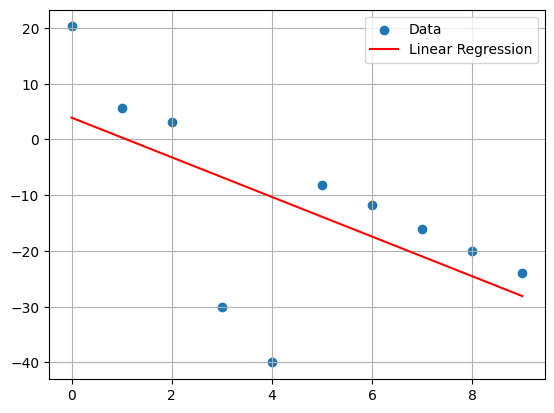
\includegraphics[width=0.685\textwidth]{resources/linear_regression_plot.png}
    \caption{\footnotesize Scatter plot of data points with fitted linear regression line}
    \label{fig:linear_regression}
\end{figure}

The fitted linear regression model is,
\begin{equation}
\hat{y} = -3.557x + 3.917
\label{eq:fitted_model}
\end{equation}

\subsection{Robust Estimator}
\begin{lstlisting}[caption={\footnotesize Robust Loss Function Implementation}]
def robust_loss(y_true, y_pred, beta):
    errors = y_true - y_pred
    return np.mean((errors**2) / (errors**2 + beta**2))
\end{lstlisting}

\subsection{Model Comparison}

Two models are evaluated using the robust estimator:
\begin{align}
\text{Model 1:} \quad y &= -4x + 12 \label{eq:model1} \\
\text{Model 2:} \quad y &= -3.55x + 3.91 \label{eq:model2}
\end{align}

\begin{lstlisting}[caption={\footnotesize Linear models}]
def model1(x): return -4*x + 12
def model2(x): return -3.55*x + 3.91
\end{lstlisting}

\begin{lstlisting}[caption={\footnotesize Robust Loss Function Implementation}]
betas = [1, 1e-6, 1e3]

for beta in betas:
    L1 = robust_loss(y, model1(x), beta)
    L2 = robust_loss(y, model2(x), beta)
    print(f"β={beta}: Model1={L1:.8f}, Model2={L2:.8f}")
\end{lstlisting}


\begin{table}[H]
\centering

\label{tab:robust_loss}
\begin{tabular}{@{}ccc@{}}
\toprule
$\beta$ Value & Model 1 Loss & Model 2 Loss \\
\midrule
$10^{-6}$ & 1.00000000 & 1.00000000 \\
$1$ & 0.43541626 & 0.97284705 \\
$10^3$ & 0.00022683 & 0.00018825 \\
\bottomrule
\end{tabular}
\caption{Robust Loss Function Values for Different $\beta$ Parameters}
\end{table}

\subsection{Optimal $\beta$ Selection}

\textbf{Analysis and Justification:}

The selection of an appropriate $\beta$ value is crucial for balancing model accuracy and outlier robustness.

\begin{itemize}
    \item \textbf{Small $\beta$ ($\beta \approx 10^{-6}$):} The loss values for both models are $1.0$, indicating that the loss function behaves almost identically for all residuals, making it highly sensitive to outliers. Thus, this setting does not help in distinguishing robust models.
    
    \item \textbf{Medium $\beta$ ($\beta = 1$):} The loss for Model 1 drops to $0.435$ while Model 2 remains high at $0.973$. This shows that the robust loss can effectively downweight the influence of outliers and favor the model that better represents the majority of the data. Hence, $\beta = 1$ provides a meaningful balance between fitting the main trend and resisting outliers.
    
    \item \textbf{Large $\beta$ ($\beta \approx 10^3$):} Both models have extremely small losses ($\sim 10^{-4}$), indicating that the influence of all residuals is almost equal. This diminishes the model discrimination and may lead to underfitting.
\end{itemize}

Based on the robust loss results, $\beta = 1$ is selected as the optimal value. It effectively distinguishes between the better-fitting model (Model 1) and a model influenced by outliers (Model 2), providing a good trade-off between accuracy and outlier robustness.


\subsection{Model Selection Using Robust Estimator}

Using the optimal $\beta = 1$, 

\textbf{Model Selection Results:}
\begin{itemize}
    \item Model 1 Loss: 0.43541626
    \item Model 2 Loss: 0.97284705
    \item Selected Model: Model 1
\end{itemize}

\textbf{Justification:} 

Using the robust loss function with $\beta = 1$, Model 1 has a significantly lower loss (0.435) compared to Model 2 (0.973). This indicates that Model 1 fits the majority of the data points more accurately while reducing the influence of extreme outliers present in the dataset. In contrast, Model 2 is more affected by the outliers, resulting in a higher robust loss. Therefore, Model 1 is selected as the preferred model as it provides a better balance between capturing the underlying trend and maintaining robustness against outliers.


\subsection{How Robust Estimator Reduces Outlier Impact}

The robust estimator reduces the influence of outliers primarily through \textbf{weighting} of residuals:
Each data point is assigned a weight based on the magnitude of its residual
\begin{equation}
w_i = \frac{1}{(y_i - \hat{y}_i)^2 + \beta^2}
\end{equation}
Large residuals, corresponding to outliers, result in smaller $w_i$, reducing their contribution to the overall loss. Conversely, residuals near the trend line retain higher weights, preserving the influence of normal data points.
This continuous weighting automatically adjusts the influence of each point based on its deviation from the model, allowing the estimator to fit the main trend without being dominated by extreme values.

\subsection{Alternative for Robust Loss Function}

An alternative loss function for robust estimation is the \textbf{Huber Loss}:

\begin{equation}
L_{\text{Huber}}(r) = \begin{cases}
\frac{1}{2}r^2 & \text{if } |r| \leq \delta \\
\delta|r| - \frac{1}{2}\delta^2 & \text{if } |r| > \delta
\end{cases}
\label{eq:huber_loss}
\end{equation}

where $r = y_i - \hat{y}_i$ and $\delta$ is a threshold parameter.

% ----------------------------------------------------------------------------------------------------
% Section 2: Loss Functions
\section{Loss Function}

% \subsubsection*{Applications and the loss functions}

% \begin{itemize}
%     \item \textbf{Application 1:} Continuous dependent variable (regression)
%     \item \textbf{Application 2:} Binary dependent variable (classification), $y \in \{0, 1\}$
% \end{itemize}

% The two loss functions:

% \begin{align}
% \text{MSE} &= \frac{1}{n} \sum_{i=1}^{n} (y_i - \hat{y}_i)^2 \label{eq:mse} \\
% \text{BCE} &= -\frac{1}{n} \sum_{i=1}^{n} [y_i \log(\hat{y}_i) + (1-y_i) \log(1-\hat{y}_i)] \label{eq:bce}
% \end{align}

\subsection{Loss Function Computation and Comparison}

For a true label $y = 1$, the loss functions are computed for various prediction values.

\begin{lstlisting}[caption={Loss Function Calculation}]
def mse(y, yhat):
    return (y - yhat)**2

def bce(y, yhat):
    return -(y*np.log(yhat) + (1-y)*np.log(1-yhat))

preds = [0.005,0.01,0.05,0.1,0.2,0.3,0.4,0.5,0.6,0.7,0.8,0.9,1.0]
results = []

for yhat in preds:
    results.append([1, yhat, mse(1,yhat), bce(1,yhat)])

df2 = pd.DataFrame(results, columns=["y","y_hat","MSE","BCE"])
df2
\end{lstlisting}

\begin{table}[H]
\centering
\caption{MSE and BCE Loss Values for Different Predictions when $y = 1$}
\label{tab:loss_comparison}
\begin{tabular}{@{}cccc@{}}
\toprule
True $y = 1$ & Prediction $\hat{y}$ & MSE & BCE \\
\midrule
1 & 0.005 & 0.990025 & 5.298317 \\
1 & 0.010 & 0.980100 & 4.605170 \\
1 & 0.050 & 0.902500 & 2.995732 \\
1 & 0.100 & 0.810000 & 2.302585 \\
1 & 0.200 & 0.640000 & 1.609438 \\
1 & 0.300 & 0.490000 & 1.203973 \\
1 & 0.400 & 0.360000 & 0.916291 \\
1 & 0.500 & 0.250000 & 0.693147 \\
1 & 0.600 & 0.160000 & 0.510826 \\
1 & 0.700 & 0.090000 & 0.356675 \\
1 & 0.800 & 0.040000 & 0.223144 \\
1 & 0.900 & 0.010000 & 0.105361 \\
1 & 1.000 & 0.000000 & NaN \\
\bottomrule
\end{tabular}
\end{table}


\newpage

\subsection{Loss Function Selection}

\subsubsection{Application 1: \textit{Loss Function:} Mean Squared Error (MSE)}

\subsubsection{Application 2: \textit{Loss Function:} Binary Cross Entropy (BCE)}

% Place for loss function plots
\begin{figure}[H]
    \centering
    \begin{subfigure}{0.49\textwidth}
        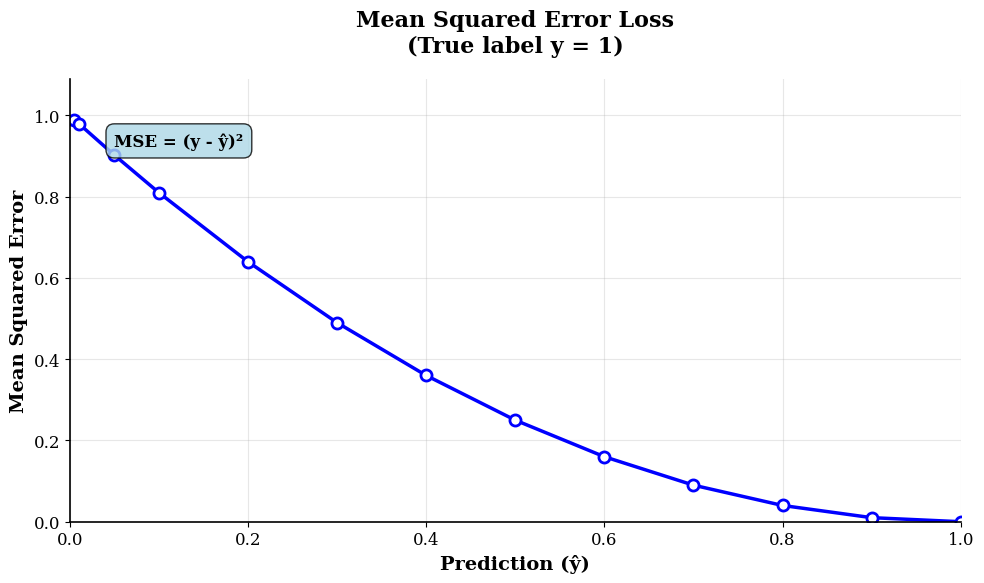
\includegraphics[width=\textwidth]{resources/MSE.png}
        \caption{MSE Loss Function}
        \label{fig:mse_plot}
    \end{subfigure}
    \hfill
    \begin{subfigure}{0.49\textwidth}
        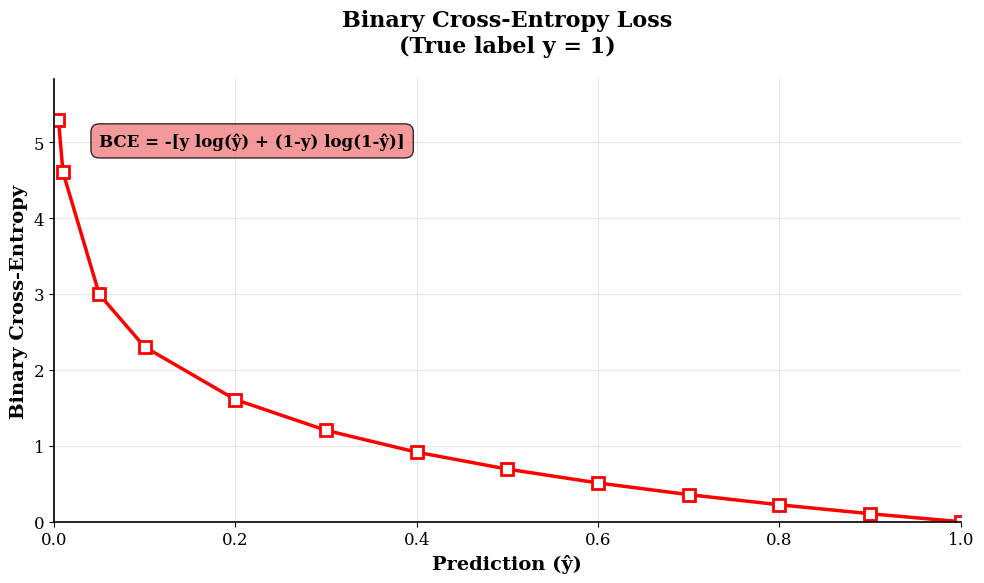
\includegraphics[width=\textwidth]{resources/BCE.png}
        \caption{BCE Loss Function}
        \label{fig:bce_plot}
    \end{subfigure}
    \caption{Individual loss function behaviors}
    \label{fig:individual_loss}
\end{figure}

\begin{figure}[H]
    \centering
    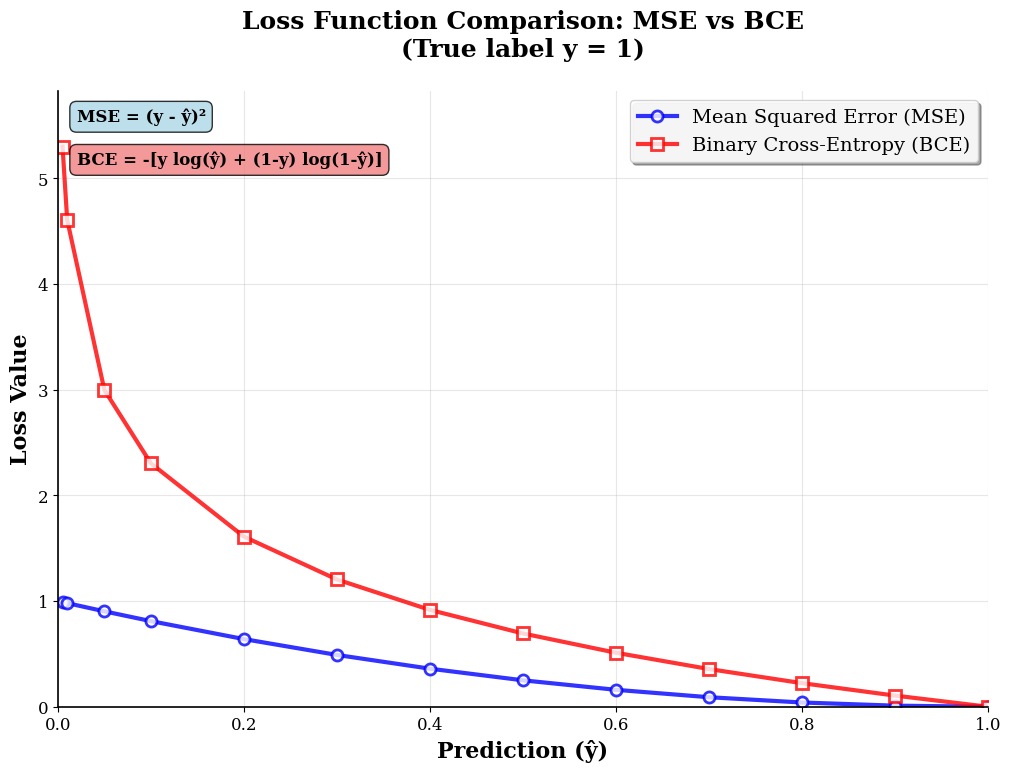
\includegraphics[width=0.8\textwidth]{resources/se_vs_bce.png}
    \caption{MSE vs BCE Loss Functions Comparison}
    \label{fig:mse_vs_bce}
\end{figure}

\vspace{0.5cm}

Looking at the computed loss values for a true label $y=1$, we can see the difference between MSE and BCE. MSE decreases gradually as the predicted value approaches 1, while BCE drops sharply, especially when predictions are close to the true label. Conversely, BCE assigns very large penalties for predictions near 0, which is desirable for classification tasks because it discourages confident wrong predictions. MSE, on the other hand, treats all deviations more uniformly, making it better suited for regression problems.

%----------------------------------------------------------------------------
\newpage

% Section 3: Data Preprocessing
\section{Data Preprocessing and Feature Scaling}

\subsection{Feature Generation}

Using the provided code, two distinct features are generated:
\subsubsection*{My Index Number: 220054N}

% Place for feature plots
\begin{figure}[H]
    \centering
    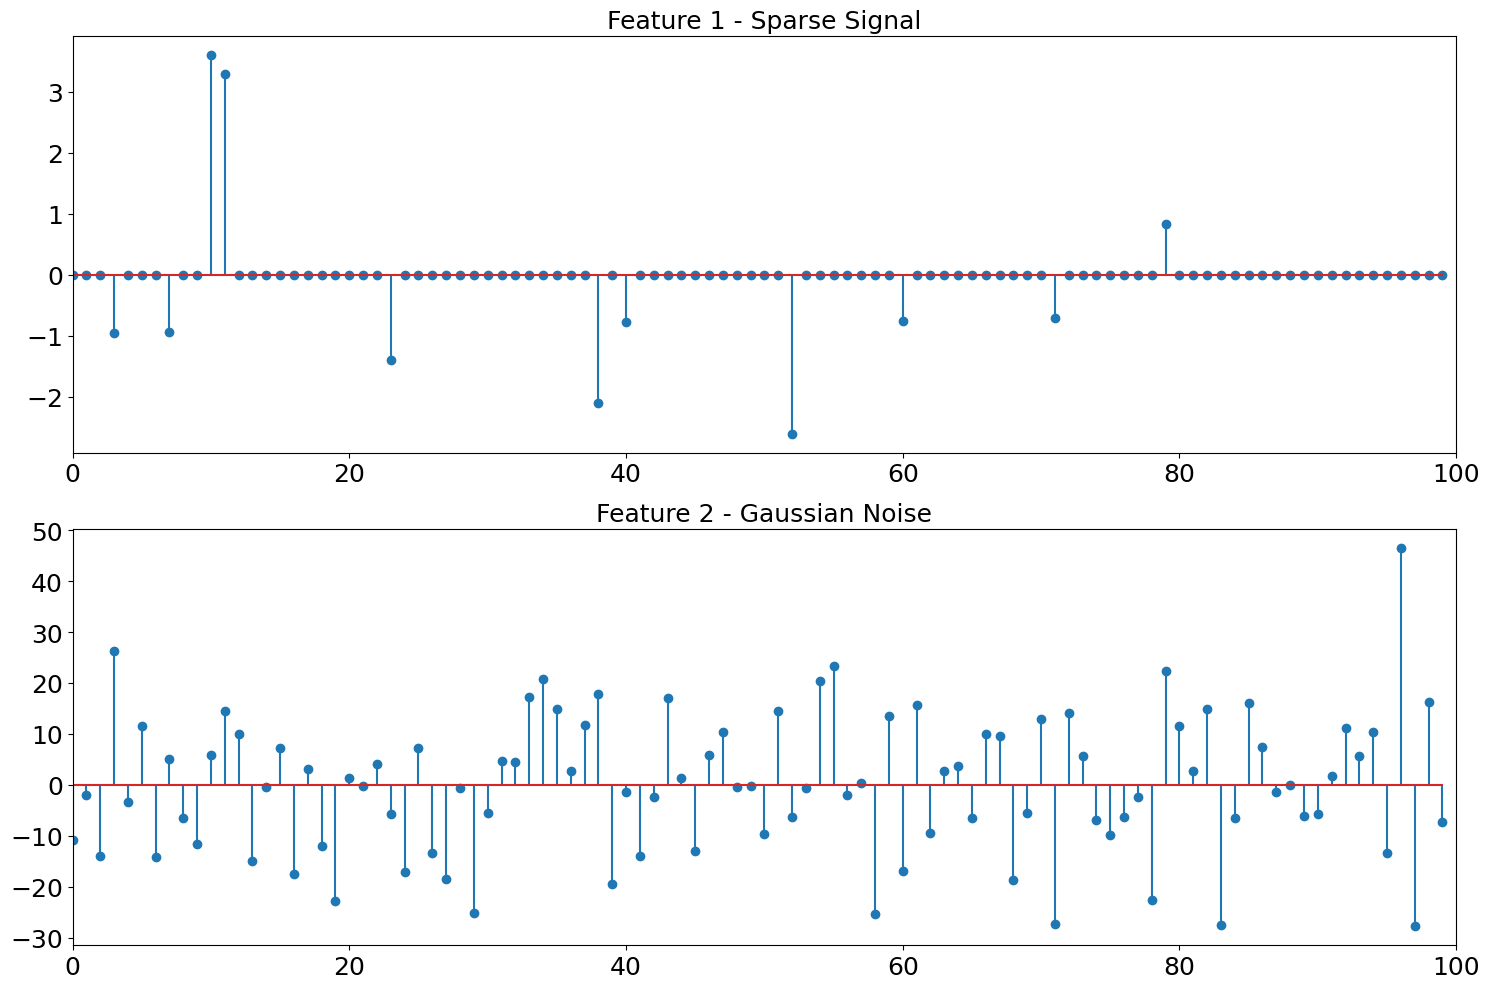
\includegraphics[width=\textwidth]{resources/features.png}
    \caption{Feature 1: Sparse Signal}
    \label{fig:feature1_original}
\end{figure}

\begin{table}[H]
\centering
\caption{Statistical Properties of Generated Features}
\label{tab:feature_stats}
\begin{tabular}{@{}lcc@{}}
\toprule
Property & Feature 1 (Sparse) & Feature 2 (Gaussian) \\
\midrule
Mean & -0.0254 & -0.0100 \\
Standard Deviation & 0.6416 & 13.5547 \\
Minimum & -2.6092 & -27.7738 \\
Maximum & 3.6000 & 46.5349 \\
Non-zero Elements & 11/100 & 100/100 \\
\bottomrule
\end{tabular}
\end{table}

\newpage
\subsection{Scaling}

\begin{enumerate}
    \item \textbf{Standard Scaling:} $x_{scaled} = \frac{x - \mu}{\sigma}$
    \item \textbf{Min-Max Scaling:} $x_{scaled} = \frac{x - x_{min}}{x_{max} - x_{min}}$
    \item \textbf{Max-Absolute Scaling:} $x_{scaled} = \frac{x}{|x|_{max}}$
\end{enumerate}

\textbf{Implementation Code:}
\begin{lstlisting}[caption={Scaling Methods Implementation}]
f1 = sparse_signal.reshape(-1,1)
f2 = epsilon.reshape(-1,1)

scalers = {
    "Standard": StandardScaler(),
    "MinMax": MinMaxScaler(),
    "MaxAbs": MaxAbsScaler()
}

fig, axes = plt.subplots(2, 3, figsize=(15, 6))  # 2 rows, 3 columns

# Feature 1 (row 0)
for col, (name, scaler) in enumerate(scalers.items()):
    scaled_f1 = scaler.fit_transform(f1)
    axes[0, col].stem(scaled_f1)
    axes[0, col].set_title(f"Feature 1 - {name}")

# Feature 2 (row 1)
for col, (name, scaler) in enumerate(scalers.items()):
    scaled_f2 = scaler.fit_transform(f2)
    axes[1, col].stem(scaled_f2)
    axes[1, col].set_title(f"Feature 2 - {name}")

plt.tight_layout()
plt.show()
\end{lstlisting}

% Place for scaling comparison plots
\begin{figure}[H]
    \centering
    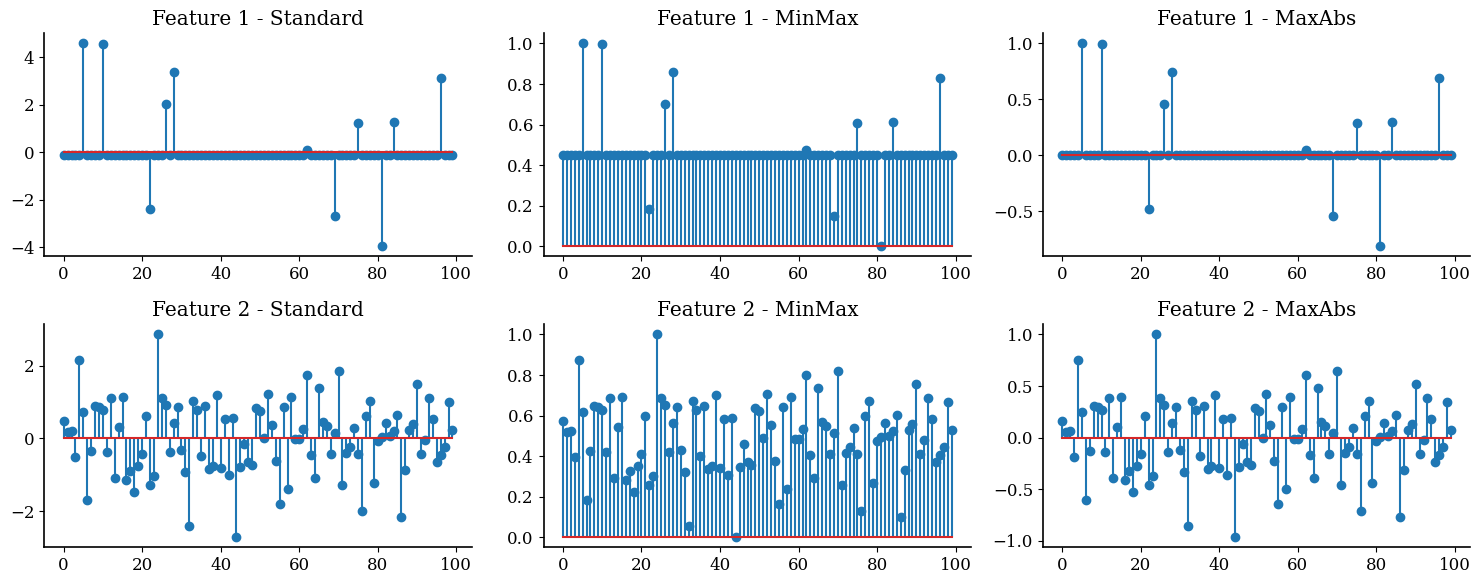
\includegraphics[width=\textwidth]{resources/scaling_comparison.png}
    \caption{Comparison of different scaling methods on both features}
    \label{fig:scaling_comparison}
\end{figure}


\begin{table}[H]
\centering
\caption{Statistical Properties After Scaling}
\label{tab:scaling_stats}
\begin{tabular}{@{}lcccccc@{}}
\toprule
\multirow{2}{*}{Method} & \multicolumn{3}{c}{Feature 1 (Sparse)} & \multicolumn{3}{c}{Feature 2 (Gaussian)} \\
\cmidrule(lr){2-4} \cmidrule(lr){5-7}
& Mean & Std & Sparsity & Mean & Std & Range \\
\midrule
Original & -0.0254 & 0.6416 & 89\% & -0.0100 & 13.5547 & 74.3087 \\
Standard & 0.0000 & 1.0000 & 0\% & 0.0000 & 1.0000 & 5.4822 \\
Min-Max & 0.4161 & 0.1033 & 0\% & 0.3736 & 0.1824 & 1.0000 \\
Max-Abs & -0.0071 & 0.1782 & 89\% & -0.0002 & 0.2913 & 1.5968 \\
\bottomrule
\end{tabular}
\end{table}


\subsubsection{Selected Scaling Methods}

\textbf{Feature 1: Max-Absolute Scaling}

\begin{itemize}
    \item Preserves sparsity by keeping exact zeros unchanged.
    \item Keeps the original structure of the signal, since it only rescales values based on the maximum absolute value.
    \item Maps all values into the range $[-1, 1]$ without shifting the mean, which is important for sparse data.
    \item Simple and efficient, as it only requires dividing by the maximum absolute value.
\end{itemize}

\textbf{Feature 2: Standard Scaling}

\begin{itemize}
    \item Normalizes the feature to have zero mean and unit variance, which matches the properties of Gaussian data.
    \item Ensures the distribution becomes standard normal, which is ideal for many statistical and machine learning models.
\end{itemize}



% ============================================================================
% REFERENCES/BIBLIOGRAPHY SECTION
% ============================================================================
% Make sure you have a 'references.bib' file with your bibliography entries
% Example entry in references.bib:
% @article{rayleigh1896sound,
%   title={The theory of sound},
%   author={Rayleigh, Lord},
%   year={1896},
%   publisher={Macmillan}
% }
% \newpage
% \addcontentsline{toc}{section}{References}    % Add References to table of contents
% \bibliographystyle{IEEEtran}                  % IEEE citation style (common in engineering)
% \bibliography{references}                      % References from references.bib file

\end{document}

% ============================================================================
% ADDITIONAL HELPFUL TIPS:
% ============================================================================
%
% 1. ADDING IMAGES:
%    - Create a 'resources' folder in your project directory
%    - Place image files there (PNG, JPG, PDF formats work well)
%    - Use \includegraphics[width=0.5\textwidth]{resources/your_image.png}
%
% 2. MATHEMATICS:
%    - Inline math: $x = y + z$
%    - Display math: \[x = y + z\]
%    - Numbered equations: \begin{equation} x = y + z \end{equation}
%
% 3. TABLES:
%    \begin{table}[H]
%    \centering
%    \begin{tabular}{|c|c|c|}
%    \hline
%    Header 1 & Header 2 & Header 3 \\
%    \hline
%    Data 1   & Data 2   & Data 3   \\
%    \hline
%    \end{tabular}
%    \caption{Your table caption}
%    \label{tab:your_label}
%    \end{table}
%
% 4. CROSS-REFERENCES:
%    - Reference figures: Figure~\ref{fig:your_label}
%    - Reference tables: Table~\ref{tab:your_label}
%    - Reference sections: Section~\ref{sec:your_label}
%
% ============================================================================
